%\documentclass[utf8x]{G7-32} % Стиль (по умолчанию будет 14pt)

\documentclass [tikz] {standalone}
\usepackage{amsmath,amssymb,amsfonts}
\usepackage{algorithmic}
\usepackage{graphicx}
\usepackage{textcomp}
\usepackage{multirow}
\usepackage{xcolor}
\usepackage{subcaption}
\usepackage{lipsum}
\usepackage{float}
\renewcommand\thesubfigure{\asbuk{subfigure}}

\usepackage{tikz}
\usepackage{pgfplots}
\usetikzlibrary{spy,calc}
\newlength\imagewidth
\newlength\imagescale
\input{header.htex}

%\usepackage[a4paper, left=-2cm, right=2cm, top=2cm, bottom=2cm]{geometry}  % Custom margins
%\pagestyle{empty}

\begin{document}



	
\begin{figure}[H]
	\centering

	\begin{subfigure}{1\textwidth}
%			\centering
		\caption{}
		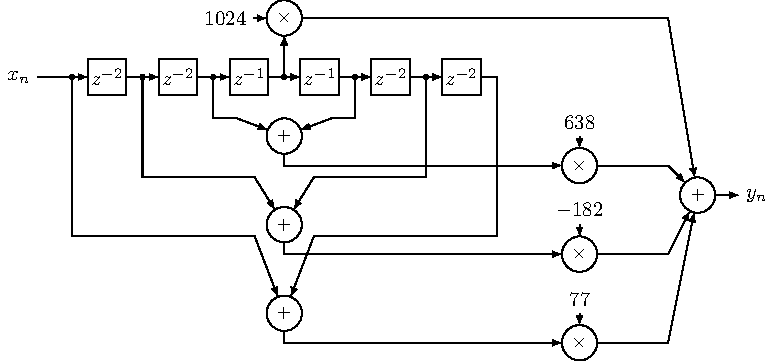
\includegraphics[width=1\linewidth]{hbf_examp_unreduced.pdf}
		\label{fig:hbf_examp_unreduced}
	\end{subfigure}%
	\vspace{0.5cm}
	\begin{subfigure}{1\textwidth}
%			\centering
		\caption{}
		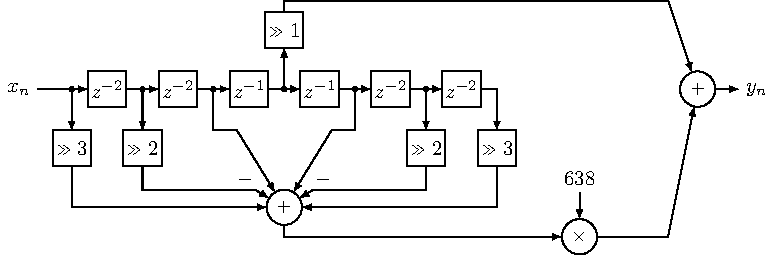
\includegraphics[width=1\linewidth]{hbf_examp_reduced.pdf}
		\label{fig:hbf_examp_reduced}
	\end{subfigure}
		\vspace{0.5cm}
%	\begin{subfigure}{1\textwidth}
%		%			\centering
%		\includegraphics[width=1\linewidth]{hbf_examp_Tmatrix.pdf}
%%		\caption{}
%		\label{fig:hbf_examp_Tmatrix}
%	\end{subfigure}
	%	\caption{(а) --- АЧХ изначального и упрощенного ППФ 30 порядка и ошибка между ними; (б) --- АЧХ изначального и упрощенного ФНЧ 94 порядка и ошибка между ними}
\end{figure}

\end{document}